\section{Funcionament general de l'aplicació web}

    \paragraph{}
    L'objectiu d'aquest apartat és explicar com els diferents components de la web interactuen entre ells per tal de crear l'aplicació web desplegada al núvol.

    Com a suport a les explicacions que s'oferiran, la figura~\ref{img:appWorkflow} mostra un diagrama amb els components principals de l'aplicació, com interactuen entre ells i els principals formats de dades que intercanvien.

    \begin{figure}
        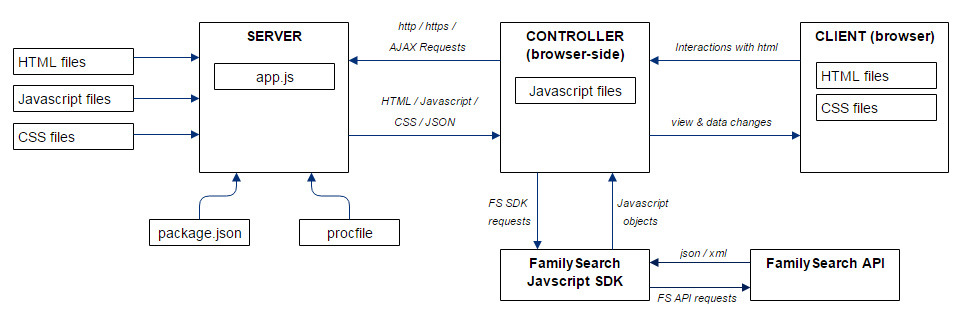
\includegraphics[scale=0.6, angle=90]{10/03_applicationWorkingFlow}
        \centering
        \caption{Comunicació entre els diferents components de l'aplicació web}\label{img:appWorkflow}
    \end{figure}

    En la imatge es poden observar les capes Servidor, Controlador i Client, que conformen l'arquitectura en tres capes explicada a la secció~\ref{sec:mvc}. També es pot observar el Javascript SDK, del que es detalla com es comunica amb l'API de FamilySearch i a quina capa de l'aplicació es troba connectat.


    \subsection{Creació del servidor}

    \paragraph{}
    L'aplicació comença a funcionar quan aquesta és executada en els servidors al núvol de Heroku, la plataforma d'hostalatge. La configuració del servidor es realitza mitjançant els fitxers \emph{Procfile} i \emph{package.json}, que s'encarreguen d'assegurar que tots els complements Javascript necessaris siguin instal·lats i s'executi el fitxer \emph{app.js} per arrancar i configurar el servidor.

    Quan la configuració del servidor acaba, aquest es troba preparat per començar a rebre peticions dels usuaris.


    \subsection{Accés a una pàgina del domini web}

    \paragraph{}
    Quan un usuari demana carregar la pàgina inicial de la nostra aplicació, una petició HTTP o HTTPS és generada i enviada cap al servidor a través del navegador del client.

    Quan el servidor la rep, l'avalua i en cas d'èxit, retorna al client els fitxers processats necessaris perquè el navegador pugui mostrar la pàgina demanada i carregar totes les funcionalitats o interaccions possibles d'aquesta al controlador.


    \subsection{Interacció amb l'API de FamilySearch}

    \paragraph{}
    El moment en què l'usuari vol interactuar amb l'API de FamilySearch, aquest es veu forçat a interactuar primer amb un element del codi HTML, per comunicar l’acció a realitzar. Per exemple, el botó de cerca de la funcionalitat d'evolució temporal d'esdeveniments.

    Quan el controlador detecta que el botó de cerca ha estat pressionat, captura l'esdeveniment i avalua la petició. En cas que no es detecti cap problema ni error en els paràmetres introduïts, el controlador realitza una crida asíncrona al SDK de FamilySearch i n'espera la resposta.

    De forma transparent a l'aplicació web, el SDK es comunica amb l’API de Family\-Search i si no hi ha cap problema en la comunicació i la petició és vàlida, aquesta retorna les dades demanades en format XML o JSON. Posteriorment, el SDK transforma la resposta de l’API en un objecte Javascript amb funcions de conveniència, que facilitaran l'accés a les dades de la resposta i el retorna al controlador.

    En el moment que el SDK retorna l'objecte, la promesa pendent de resolució que havia creat el controlador és resolta i l'objecte retornat pel SDK passa a ser accessible. Arribats a aquest punt, el controlador processa i transforma les dades contingudes a l'objecte de la forma desitjada i un cop finalitzades les operacions necessàries, modifica la vista del client introduint els canvis pertinents en aquesta.


    \subsection{Interacció amb elements del HTML}

    \paragraph{}
    Quan els usuaris interactuen amb elements bàsics del HTML, per exemple, quan interactuen amb les caixes que permeten expandir o plegar seccions del formulari en les funcionalitats de cerca o evolució geogràfica de cognoms, la resposta a realitzar per part del controlador és bastant simple.

    En el moment que el controlador detecta que s'ha interactuat amb algun dels elements que escolta, captura l'esdeveniment, avalua com s'ha de procedir segons el context de l'acció (en el cas de l’exemple, plegar o desplegar contingut d'un formulari) i realitza de forma immediata els canvis a la vista del navegador.


    \subsection{Conclusió}

    \paragraph{}
    Els casos d'ús que s'han cobert en els apartats anteriors són relativament simples, però són una mostra representativa del conjunt d'accions diferents a les quals l'aplicació pot haver de fer front.

    Esperem que aquesta secció hagi servit per il·lustrar el funcionament general de la web i com els diferents components interactuen entre ells. La resta d’accions possibles en el web, requerint més o menys complexitat per part del controlador, segueixen una de les tres rutes descrites en els apartats anteriors per tal de ser satisfetes.
